% =============================================================
%  Urban Waste Detection — WVC/IEEE conference format (2 col.)
%  Compile: pdflatex main && bibtex main && pdflatex main ×2
% =============================================================
\documentclass[conference]{IEEEtran}

\usepackage[utf8]{inputenc}
\usepackage[T1]{fontenc}
\usepackage{graphicx}
\usepackage{booktabs}
\usepackage{multirow}
\usepackage{amsmath}
\usepackage{xcolor}
\usepackage[colorlinks=true, citecolor=blue, urlcolor=blue, linkcolor=blue]{hyperref}
\usepackage{tikz}
\usetikzlibrary{positioning, arrows.meta}

\graphicspath{{../figuras_final/}{../figuras_eda/}{../figuras_p0/}{../figuras_p1/}}

% Result placeholders: highlighted until notebook 06 numbers land
\newcommand{\PEND}[1]{\textcolor{red}{\textbf{[#1]}}}

\begin{document}

\title{How Far Does a Litter Detector Travel?\\
Cross-Domain Urban Waste Detection Across Handheld, Dashcam and Drone Imagery}

\author{
\IEEEauthorblockN{Jairzinho Santos}
\IEEEauthorblockA{Universidad Nacional de Ingenier\'ia \\
Lima, Peru \\
Computer Vision, MSc in Artificial Intelligence \\
2026-I}}

\maketitle

% =============================================================
\begin{abstract}
% <= 150 words
Automated litter monitoring is usually evaluated within a single imaging domain,
yet real deployments mix handheld reports, vehicle cameras and drones. We study
how much urban waste detectors degrade across three public domains TACO
(handheld), RoLID-11K (dashcam) and UAVVaste (drone) under a single audited
evaluation protocol. Our curation uncovered seven defects in the released
datasets, most notably video-level leakage in RoLID-11K's official splits, where
58.2\% of test images share a source video with training; a model trained with
that overlap scores +21\% AP$_{50}$ on the same test set. We compare Faster
R-CNN, an FCN segmenter and CAM-based interpretability against a YOLOv11
reference, and measure a cross-domain degradation of 82\% mAP$_{50}$, dominated
by object scale (median 22\,px in dashcam imagery, below the smallest FPN
anchor). Raising input resolution to 1024\,px recovers up to 8.3 AP$_{50}$ and
5.8 AP$_S$ points. Code, weights and audited splits are released.
\end{abstract}

\begin{IEEEkeywords}
litter detection, cross-domain evaluation, dataset auditing, small objects
\end{IEEEkeywords}

% =============================================================
\section{Introduction}
Uncollected urban waste harms public health, tourism and municipal budgets, and
its monitoring still relies on manual inspection with limited coverage. Computer
vision promises continuous, low-cost monitoring, and recent work has produced
public datasets for litter detection in complementary settings: street-level
handheld photographs (TACO~\cite{taco}), forward-facing dashcams
(RoLID-11K~\cite{rolid}), drone imagery (UAVVaste~\cite{uavvaste}) and waste-truck
fisheye cameras (StreetView-Waste~\cite{streetview}). Each benchmark, however, is
evaluated \emph{in-domain}; whether a detector trained on one viewpoint remains
useful on another the situation any city deploying mixed sensors faces has
not been measured.

This paper asks: \emph{how much does urban litter detection degrade across
imaging domains, and what matters most to close the gap architecture, input
resolution, or training data hygiene?} Answering it required more than training
detectors. Auditing the three datasets surfaced seven defects (Section~\ref{sec:data}),
including video-level leakage in RoLID-11K's official splits that inflates
published baselines, basename collisions and inconsistent EXIF annotation frames
in TACO and UAVVaste. We therefore built an audited curation pipeline with frozen,
group-aware splits, and evaluate every model against the same ground truths.

Our contributions are:
(i) a documented audit of three public litter datasets, with corrected and
released splits;
(ii) the first cross-domain evaluation matrix across handheld, dashcam and drone
litter imagery;
(iii) a quantification of the leakage inflation in RoLID-11K's official protocol
(+21\% AP$_{50}$ from scene memorization);
(iv) a controlled comparison of classical fine-tuned detectors, segmentation and
interpretability techniques against a modern real-time reference, including a
small-object resolution ablation and a class-granularity (6 vs.\ 5 material
classes) study.

% =============================================================
\section{Related Work}
\textbf{Litter datasets.} TACO~\cite{taco} provides 1{,}500 handheld images with
60 litter categories and segmentation polygons. RoLID-11K~\cite{rolid} contributes
11.5k dashcam frames with a single \emph{litter} class and pronounced small-object
statistics. UAVVaste~\cite{uavvaste} covers low-altitude drone views.
StreetView-Waste~\cite{streetview} targets waste-truck fisheye cameras; its
download endpoints were unavailable during this work.
Detect-waste~\cite{detectwaste} harmonized several of these sources; ZeroWaste~\cite{zerowaste}
addresses industrial sorting, a domain we deliberately exclude.

\textbf{Detection under constraints.} TrashDet~\cite{trashdet} searches TinyML
detectors on TACO, reaching 19.5 mAP$_{50}$ on a five-class subset evidence that
absolute scores in this problem are structurally low, which motivates our focus on
\emph{relative} cross-domain quantities. RoLID's authors benchmark modern
detectors, with transformer heads (CO-DETR) leading YOLO variants by over
20 AP$_{50}$ points, consistent with the extreme small-object regime.

\textbf{Methods.} We build on Faster R-CNN~\cite{fasterrcnn} and its RPN, fully
convolutional segmentation~\cite{fcn}, class-activation
interpretability~\cite{cam,gradcam,guidedbp}, YOLOv11~\cite{yolo11} as the
real-time reference, TIDE~\cite{tide} for error decomposition and iterative
stratification~\cite{sechidis} for group-aware splitting.

% =============================================================
\section{Datasets, Audit and Curation}
\label{sec:data}

We ingest the three in-scope datasets through a medallion pipeline
(raw$\rightarrow$bronze$\rightarrow$silver$\rightarrow$gold) with per-layer
manifests and SHA-256 lineage; Figure~\ref{fig:pipeline} overviews the whole
flow, from verified ingestion to the evaluation contract.

\begin{figure*}[t]
\centering
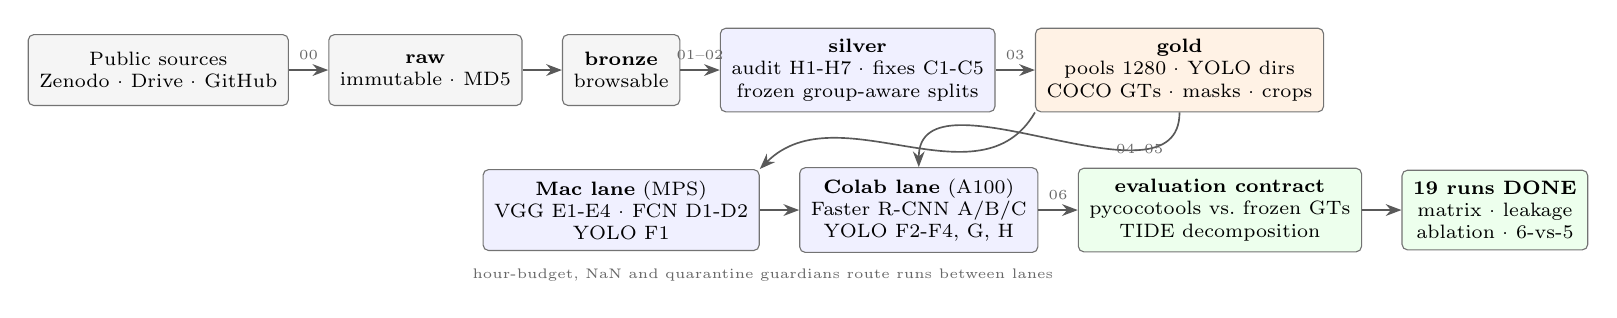
\begin{tikzpicture}[
  caja/.style={draw=black!55, rounded corners=2pt, align=center,
               font=\scriptsize, inner sep=4pt, minimum height=9mm},
  fl/.style={-{Stealth[length=2mm]}, black!65, semithick},
  et/.style={font=\tiny, black!60},
  node distance=5mm and 5mm]
\node[caja, fill=black!4] (src) {Public sources\\Zenodo · Drive · GitHub};
\node[caja, fill=black!4, right=of src] (raw) {\textbf{raw}\\immutable · MD5};
\node[caja, fill=black!4, right=of raw] (bronze) {\textbf{bronze}\\browsable};
\node[caja, fill=blue!6, right=of bronze] (silver) {\textbf{silver}\\audit H1-H7 · fixes C1-C5\\frozen group-aware splits};
\node[caja, fill=orange!10, right=of silver] (gold) {\textbf{gold}\\pools 1280 · YOLO dirs\\COCO GTs · masks · crops};
\node[caja, fill=blue!6, below=8mm of bronze] (mac) {\textbf{Mac lane} (MPS)\\VGG E1-E4 · FCN D1-D2\\YOLO F1};
\node[caja, fill=blue!6, right=of mac] (colab) {\textbf{Colab lane} (A100)\\Faster R-CNN A/B/C\\YOLO F2-F4, G, H};
\node[caja, fill=green!7, right=of colab] (eval) {\textbf{evaluation contract}\\pycocotools vs.\ frozen GTs\\TIDE decomposition};
\node[caja, fill=green!7, right=of eval] (res) {\textbf{19 runs DONE}\\matrix · leakage\\ablation · 6-vs-5};
\draw[fl] (src) -- node[et, above]{00} (raw);
\draw[fl] (raw) -- (bronze);
\draw[fl] (bronze) -- node[et, above]{01--02} (silver);
\draw[fl] (silver) -- node[et, above]{03} (gold);
\draw[fl] (gold.south) to[out=-90, in=90] node[et, right, pos=0.35]{04--05} (colab.north);
\draw[fl] (gold.south west) to[out=-120, in=45] (mac.north east);
\draw[fl] (mac) -- (colab);
\draw[fl] (colab) -- node[et, above]{06} (eval);
\draw[fl] (eval) -- (res);
\node[et, below=1mm of mac.south, xshift=18mm]
  {hour-budget, NaN and quarantine guardians route runs between lanes};
\end{tikzpicture}
\caption{End-to-end pipeline. Data flows through a medallion architecture with
SHA-256 lineage (arrow labels: notebook numbers); training runs on two lanes
governed by automatic guardians; every model is evaluated under a single metric
contract.}
\label{fig:pipeline}
\end{figure*}
 Table~\ref{tab:domains} summarizes the domains and Figure~\ref{fig:scale} shows the axis that separates them: object scale.

\begin{table}[t]
\caption{The three domains after curation. Median object side measured on the
original images; at the 640-px training resolution these become $\sim$32,
$\sim$7 and $\sim$12\,px respectively.}
\label{tab:domains}
\centering
\small
\begin{tabular}{lcccc}
\toprule
Dataset & Viewpoint & Images & Median obj. & \% small \\
\midrule
TACO & handheld & 1{,}500 & 171 px & 25 \\
RoLID-11K & dashcam & 11{,}564 & \textbf{22 px} & 84 \\
UAVVaste & drone & 772 & 72 px & 66 \\
\bottomrule
\end{tabular}
\end{table}

\begin{figure}[t]
\centering
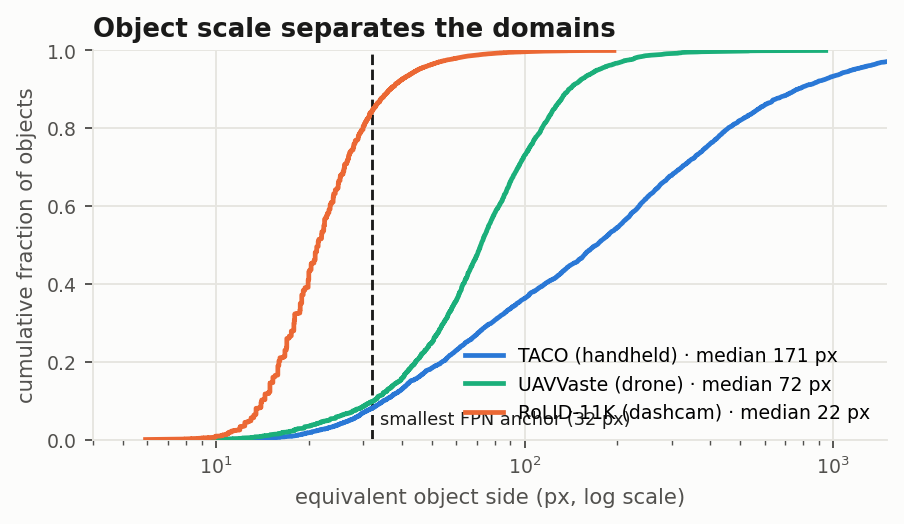
\includegraphics[width=\linewidth]{escala_objetos_en.png}
\caption{Cumulative distribution of object side per domain. RoLID's
median (22\,px) falls below the smallest 32-px FPN anchor: the regime
that explains the cross-domain matrix and motivates the resolution
ablation.}
\label{fig:scale}
\end{figure}


\textbf{Audit findings.} Systematic checks (perceptual hashing, EXIF-frame
verification, split cross-referencing) surfaced seven defects we correct or
document: (H1) TACO basenames collide across batches (92\% of images share a
filename with another batch); (H2) $\sim$37\% of TACO images carry pending EXIF
rotations, with boxes annotated on the \emph{rotated} frame; (H3) RoLID's release
folders do not encode capture hour; (H4) \textbf{RoLID's official splits leak at
the video level}: 22 of 84 source videos span multiple splits and 58.2\% of test
frames share a video with training near-duplicate frames (87\% visual
redundancy by perceptual hash) make this scene leakage, inflating published
baselines; (H5) one image is duplicated between official val and test; (H6)
UAVVaste's official split also contains one near-duplicate pair across
train/test; (H7) annotation frames are inconsistent across datasets TACO
annotates on the EXIF-rotated frame while five UAVVaste handheld photos annotate
the raw frame so pixels are materialized per-image in the frame that matches
the declared dimensions, with EXIF metadata stripped.

\textbf{Curation.} Silver applies five corrections (duplicate removal from val,
phantom-category removal, full-path identity, degenerate-box and MD5 flags),
defines a two-level taxonomy \emph{litter} (1 class, all datasets) and TACO
material classes in two parallel variants, \textbf{A: 6 classes} (glass included,
marginal at 38 projected test instances) and \textbf{B: 5 classes} (glass
excluded) and freezes four split schemes with group-aware units: pHash visual
groups for TACO/UAVVaste and \emph{source video} for RoLID. TACO splits use
iterative stratification~\cite{sechidis}; every class lands within 0.1\,pp of the
15\% test target. For RoLID we keep \emph{both} the official (leaky, for
comparability) and a by-video (0\% leakage) scheme, enabling a paired
quantification of the inflation.

% =============================================================
\section{Methods}
\label{sec:methods}

\textbf{P0 - fine-tuned classical pipeline.}
(1)~\emph{Faster R-CNN} (ResNet-50-FPN, COCO-pretrained) under two transfer
strategies frozen backbone vs.\ unfreezing \texttt{layer4} with linear warmup,
gradient clipping and early stopping on validation AP$_{50}$.
(2)~\emph{FCN-ResNet18} for binary litter/background segmentation on TACO's
rasterized polygons ($1\times1$ conv + $\times$32 transposed conv with bilinear
init, class-weighted cross-entropy).
(3)~\emph{VGG-16 transfer learning} on 224-px litter/background crops (two
strategies $\times$ two learning rates), providing the substrate for
CAM~\cite{cam}, Grad-CAM~\cite{gradcam} and Guided Backpropagation~\cite{guidedbp}
interpretability panels.
(4)~An \emph{anchor-coverage analysis}: FPN base anchors (32-512 px) against the
measured object-size distributions, plus RPN objectness maps from the trained
dashcam model a mechanistic account of the small-object gap.

\textbf{P1 - modern reference.} YOLOv11n~\cite{yolo11} trained per domain at
640 px (and 1024 px for the resolution ablation), used to fill the $3\times3$
cross-domain matrix, the official-vs-by-video leakage pair, and the 6-vs-5-class
variant comparison.

\textbf{Evaluation contract.} A single source of metric truth: predictions from
every model are evaluated with COCO tooling against the same frozen ground
truths; test is touched once per experiment with best-validation weights; saved
predictions feed TIDE~\cite{tide} error decomposition.

% =============================================================
\section{Experimental Setup}
Nineteen runs (11 P0, 8 P1) executed on two lanes: Apple M-series (MPS) for
VGG/FCN/YOLO and CUDA (Colab A100) for Faster R-CNN and the heavier YOLO
runs profiling showed healthy Faster R-CNN iterations cost $\sim$95\,s on MPS
(variable input shapes force per-shape kernel recompilation), versus
$\sim$0.3\,s on CUDA; an hour-budget guardian projected total cost after the
first epoch and routed unviable runs automatically. Budgets: generous epoch caps
(50-150) with early stopping (patience 8-30) and validation curves; seeds
fixed; per-epoch checkpoints with resume. Images are materialized at max side
1280 (Lanczos, JPEG q95) in the annotation frame (H7). Figure~\ref{fig:curves} shows the validation trajectories of the eight
YOLO runs: clean convergence, early stopping at work, and the separation
by domain and resolution.

\begin{figure}[t]
\centering
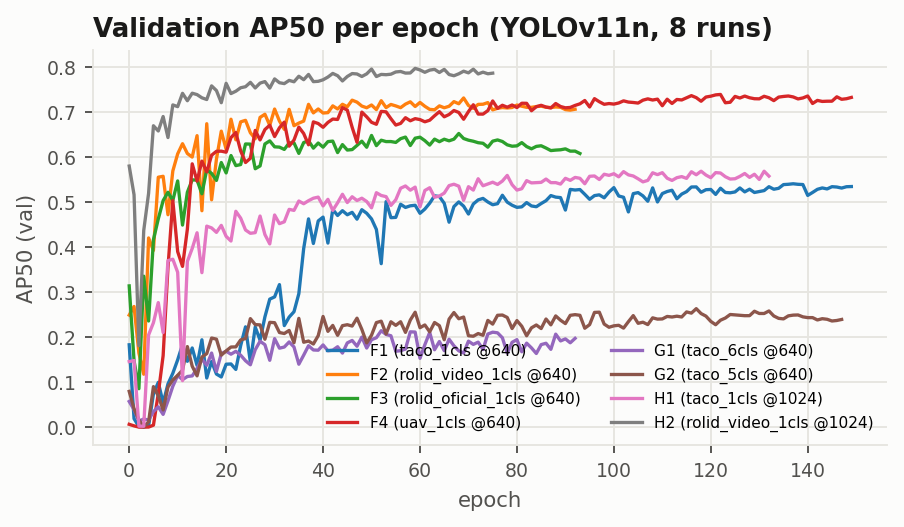
\includegraphics[width=\linewidth]{p1_curvas_en.png}
\caption{Validation AP$_{50}$ per epoch for the eight YOLOv11n runs.}
\label{fig:curves}
\end{figure}

Multiclass exports
exclude \emph{poisoned negatives} images whose only objects belong to excluded
classes rather than training them as background (1/38/60 images for the
1/6/5-class variants).

% =============================================================
\section{Results}
\label{sec:results}
Every number below is generated by the consolidated evaluation notebook from
saved test predictions against the frozen ground truths; no metric is
transcribed by hand.

\subsection{Cross-domain matrix}
Figure~\ref{fig:matrix} presents the central result. In-domain, the three
YOLOv11n models average 0.639 AP$_{50}$; across domains this collapses to
0.118 an \textbf{82\% degradation}. The matrix is strongly asymmetric: the
dashcam domain is an island (AP$_{50}\!\le\!0.064$ in either direction), while
handheld$\rightarrow$drone transfers surprisingly well (0.527, retaining 68\% of
the drone in-domain score). This pattern indicts \emph{object scale} rather than
appearance alone: TACO and UAVVaste objects (median 171 and 72\,px) both lie
within the FPN anchor range, whereas RoLID's 22-px median falls below the
smallest 32-px anchor consistent with our anchor-coverage analysis and with
AP$_S$ collapsing hardest (diagonal AP$_S$: 0.056 / 0.279 / 0.374).

\begin{figure}[t]
\centering
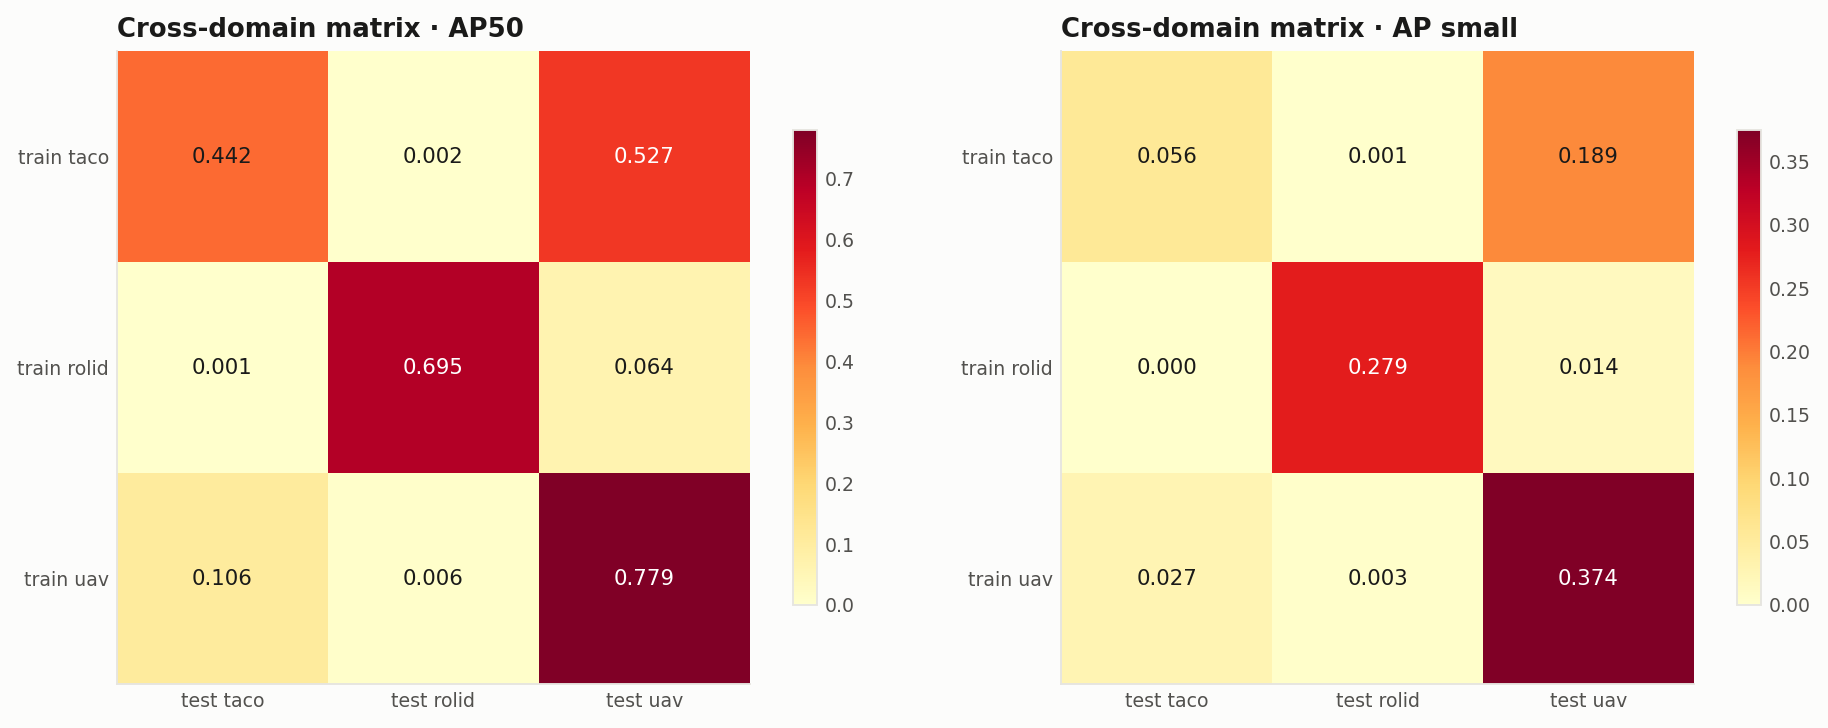
\includegraphics[width=\linewidth]{matriz_cross_domain_final_en.png}
\caption{Cross-domain matrix on test (YOLOv11n @640): AP$_{50}$ (left)
and AP$_S$ (right). Rows: training domain; columns: test domain.
In-domain mean 0.639 vs.\ cross-domain 0.118.}
\label{fig:matrix}
\end{figure}

\subsection{Leakage inflation in RoLID-11K}
Table~\ref{tab:leak} pairs the official (58\% video leakage) and by-video (0\%)
protocols. On the \emph{same} clean by-video test set, the model trained on the
official split which saw other frames of those very test videos scores
0.844 AP$_{50}$ versus 0.695 for the cleanly trained model: a \textbf{+21\%
relative inflation} attributable to scene memorization, not generalization
(87\% of intra-video frame pairs are visually redundant by perceptual hash).
Published baselines on the official protocol should be read with this bias in
mind; group-aware splitting removes it at zero cost.

\begin{table}[t]
\caption{Leakage quantification on RoLID-11K (test AP$_{50}$, YOLOv11n @640).}
\label{tab:leak}
\centering
\small
\begin{tabular}{llc}
\toprule
Training split & Test set & AP$_{50}$ \\
\midrule
official (58\% leak) & official & 0.620 \\
by-video (0\% leak) & by-video & 0.695 \\
official (58\% leak) & by-video & \textbf{0.844} \\
\bottomrule
\end{tabular}
\end{table}

\subsection{Families under the same protocol}
Table~\ref{tab:families} compares Faster R-CNN (41.3\,M parameters) and
YOLOv11n (2.6\,M) on identical splits and ground truths. On single-class tasks
the 16$\times$ smaller model stays within 1-4 AP$_{50}$ points (0.695 vs.\
0.707 on dashcam; 0.442 vs.\ 0.483 on handheld), supporting lightweight
deployment; on material classification the gap widens to 5-9 points.
Unfreezing \texttt{layer4} lifts Faster R-CNN by +3.7 AP$_{50}$ over the frozen
backbone (0.483 vs.\ 0.446). Our 5-class YOLO (0.192 mAP$_{50}$) is consistent
with TrashDet's 19.5 on a comparable TACO subset~\cite{trashdet}, confirming
that absolute scores in this problem are structurally low. The complementary P0
models complete the picture: FCN-ResNet18 reaches 0.577 test IoU on binary
litter segmentation, and the VGG-16 crop classifier attains 97.8\% test
accuracy, providing the substrate for the CAM/Grad-CAM evidence that the
network attends to the object rather than context (Figure~\ref{fig:cam}).

\begin{figure}[t]
\centering
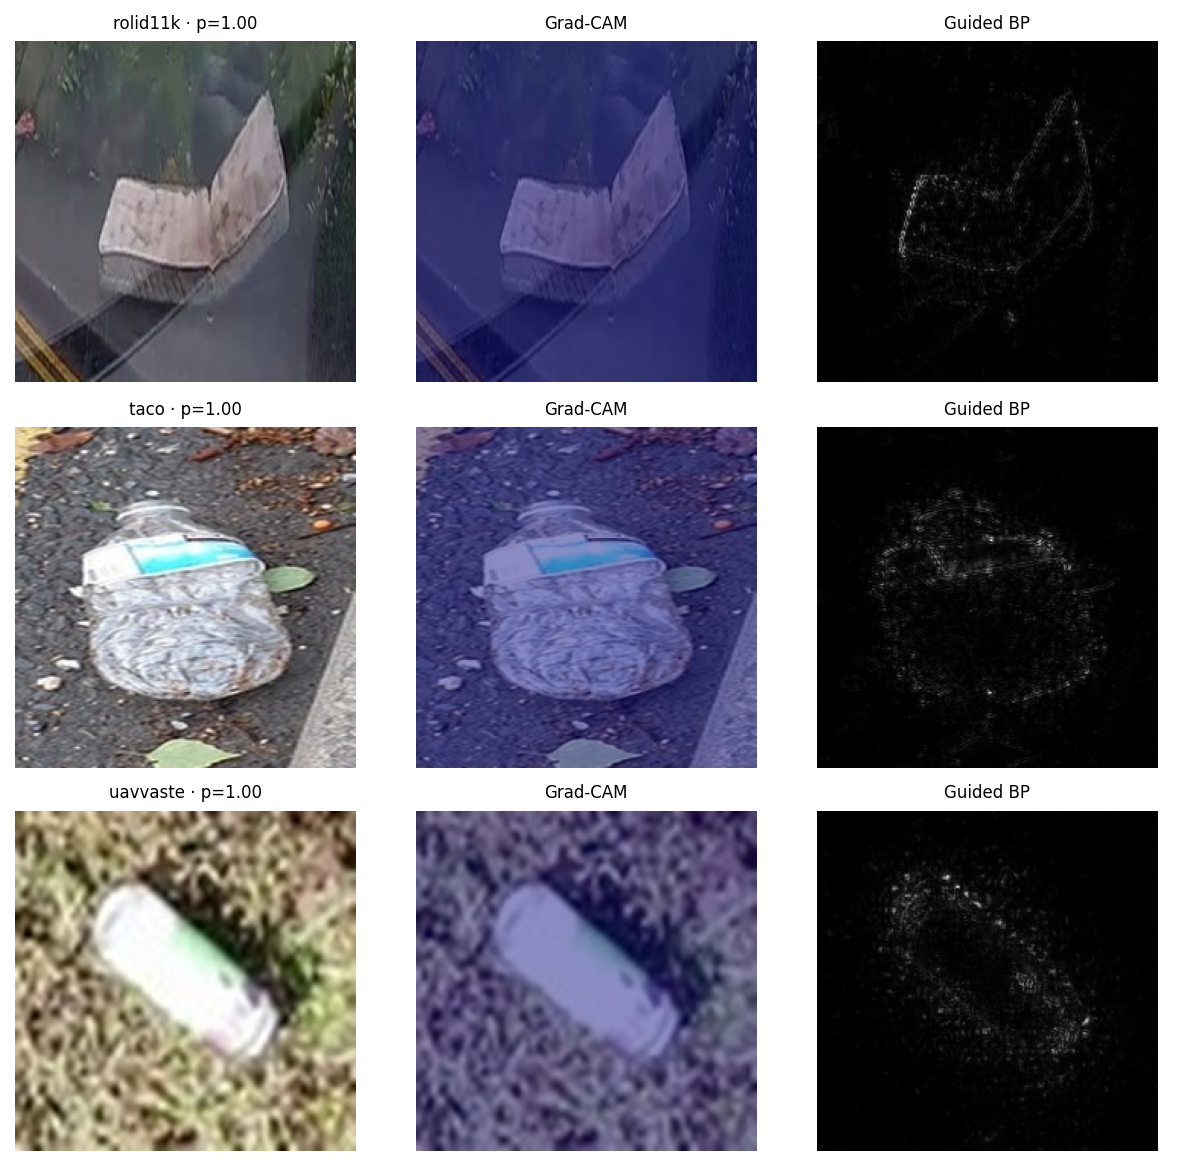
\includegraphics[width=\linewidth]{cam_panel_paper.png}
\caption{Crop-classifier interpretability: one row per domain (dashcam,
handheld, drone) with Grad-CAM and Guided Backpropagation. Activation
concentrates on the object even in 22-px crops.}
\label{fig:cam}
\end{figure}

\begin{table}[t]
\caption{Model families on identical splits (test metrics). FRCNN = Faster
R-CNN R50-FPN, \texttt{layer4} unfrozen.}
\label{tab:families}
\centering
\small
\begin{tabular}{llccc}
\toprule
Data & Model & AP$_{50}$ & AP & AP$_S$ \\
\midrule
\multirow{2}{*}{TACO 1-cls} & FRCNN & \textbf{0.483} & \textbf{0.323} & \textbf{0.073} \\
 & YOLOv11n & 0.442 & 0.318 & 0.056 \\
\midrule
\multirow{2}{*}{RoLID by-video} & FRCNN & \textbf{0.707} & 0.277 & \textbf{0.281} \\
 & YOLOv11n & 0.695 & \textbf{0.279} & 0.279 \\
\midrule
\multirow{2}{*}{TACO 6-cls} & FRCNN & \textbf{0.246} & 0.154 & 0.029 \\
 & YOLOv11n & 0.157 & - & - \\
\midrule
\multirow{2}{*}{TACO 5-cls} & FRCNN & \textbf{0.244} & 0.155 & 0.024 \\
 & YOLOv11n & 0.192 & - & - \\
\bottomrule
\end{tabular}
\end{table}

\subsection{Resolution and class granularity}
Table~\ref{tab:res} shows the 640$\rightarrow$1024 ablation. Gains concentrate
exactly where objects are smallest: +8.3 AP$_{50}$ and +5.8 AP$_S$ on dashcam,
versus +3.2 and +3.9 on handheld resolution is the cheapest effective lever
for the small-object regime. For class granularity, excluding the marginal
glass class (38 test instances, AP$_{50}$ 0.049 when kept) improves the global
5-class score to 0.192 vs.\ 0.157 for 6 classes, with a mean +0.014 AP$_{50}$
on the five shared classes (largest on metal, +0.077): keeping a
severely under-represented class taxes its siblings.

\begin{table}[t]
\caption{Resolution ablation (YOLOv11n, test).}
\label{tab:res}
\centering
\small
\begin{tabular}{lcccc}
\toprule
 & \multicolumn{2}{c}{AP$_{50}$} & \multicolumn{2}{c}{AP$_S$} \\
Domain & 640 & 1024 & 640 & 1024 \\
\midrule
TACO & 0.442 & \textbf{0.474} & 0.056 & \textbf{0.096} \\
RoLID & 0.695 & \textbf{0.779} & 0.279 & \textbf{0.337} \\
\bottomrule
\end{tabular}
\end{table}

\subsection{Error decomposition}
Figure~\ref{fig:tide} decomposes the error with TIDE across all 13 detectors.
Three regimes emerge. Multiclass models are dominated by \emph{classification}
error (up to 24.6 dAP in the 5-class YOLO, against only 1.7 for localization):
finding litter is not the bottleneck naming its material is. Single-class
handheld models split their error between background false positives and
missed objects ($\sim$11-13 dAP each). In-domain dashcam models,
counter-intuitively, miss little (dAP$_{\text{Miss}}\!\le\!3.9$): the 22-px
objects \emph{are} found, and the residual error is dominated by background
confusions evidence that the cross-domain collapse of Figure~\ref{fig:matrix}
stems from representations, not from an unrecoverable recall floor.

\begin{figure}[t]
\centering
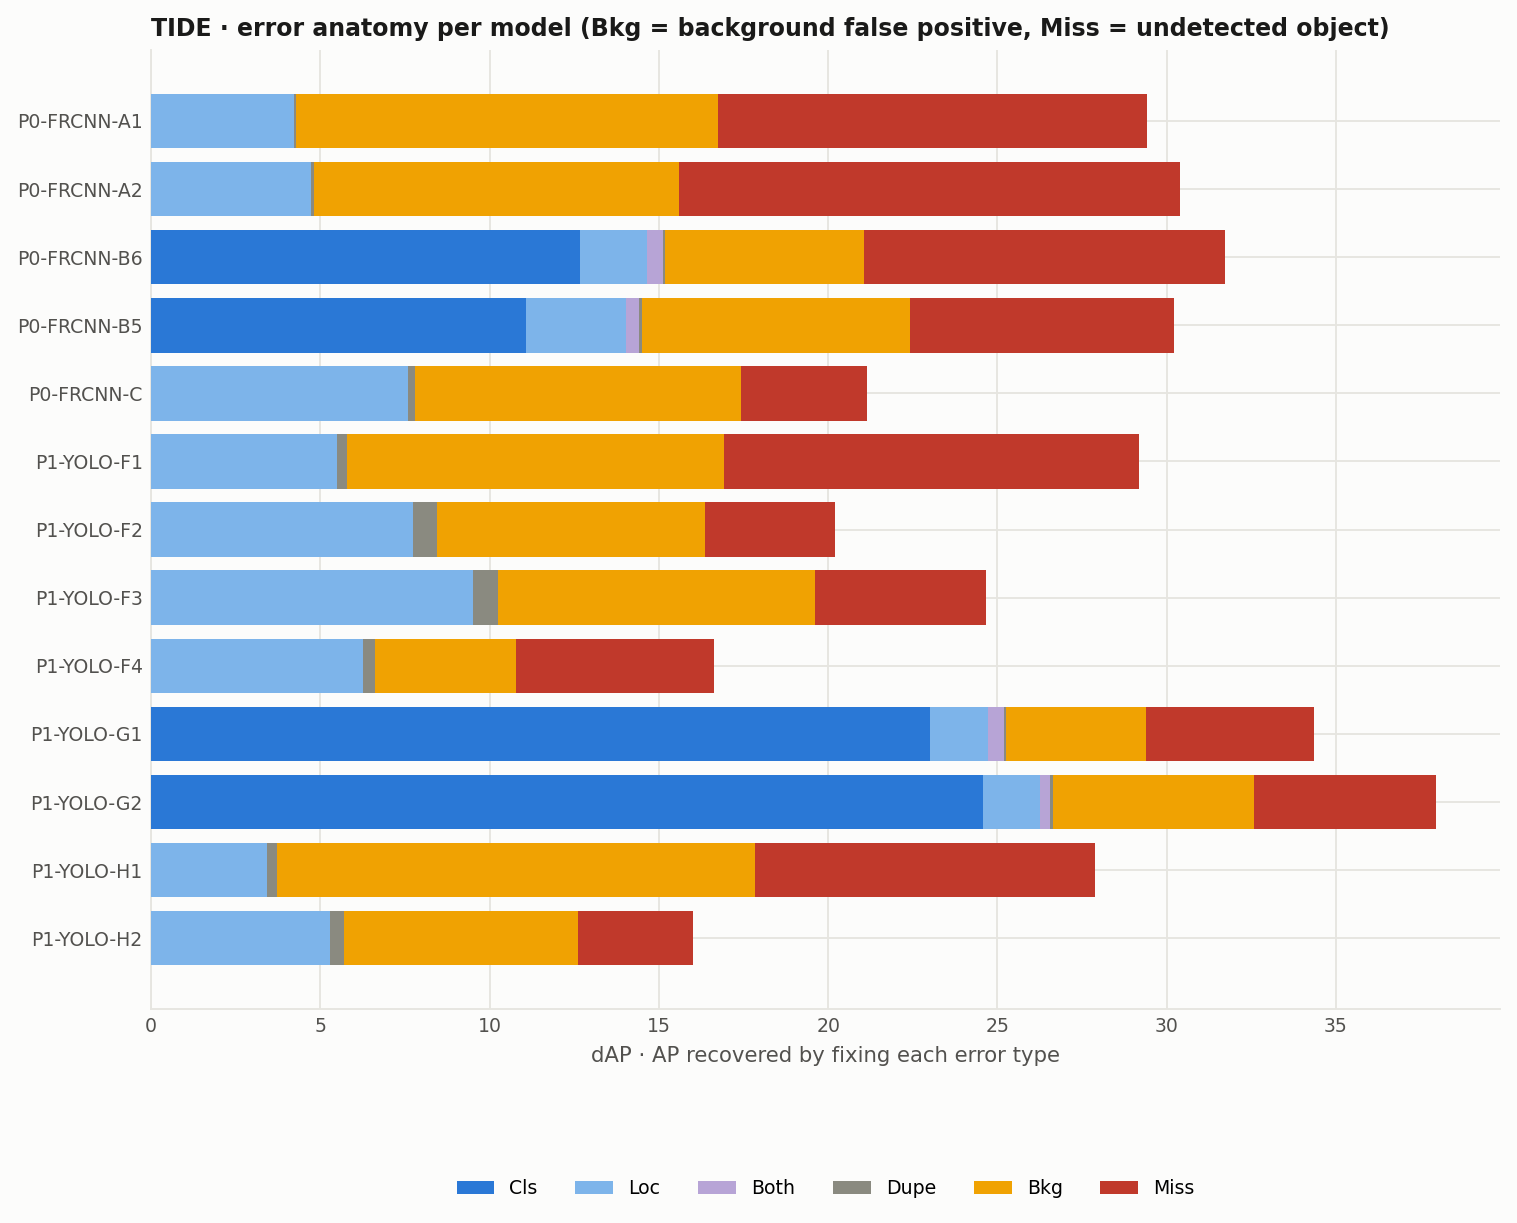
\includegraphics[width=\linewidth]{tide_descomposicion_en.png}
\caption{TIDE error decomposition per model (dAP recovered by fixing each error
type). Cls dominates multiclass models; Bkg+Miss dominate single-class ones.}
\label{fig:tide}
\end{figure}

\subsection{Qualitative out-of-distribution results}
Figure~\ref{fig:demo} shows the batched demo (notebook 07) on a session of ten
images downloaded from the internet, unrelated to the three datasets. Under
conservative thresholds (0.25 for YOLO, 0.5 for Faster R-CNN), the quantitative
patterns reappear out of distribution: Faster R-CNN proposes more candidates
than YOLOv11n on all ten images (211 vs.\ 87 detections in total; 45 vs.\ 15 on
the densest scene), the FCN estimates 3-16\% litter pixels per scene, and the
VGG classifier confirms every crop with P(litter)$\ge$0.99, Grad-CAM attending
to the object rather than its context. These images are illustrative evidence,
not a metric: they carry no annotations.

\begin{figure*}[t]
\centering
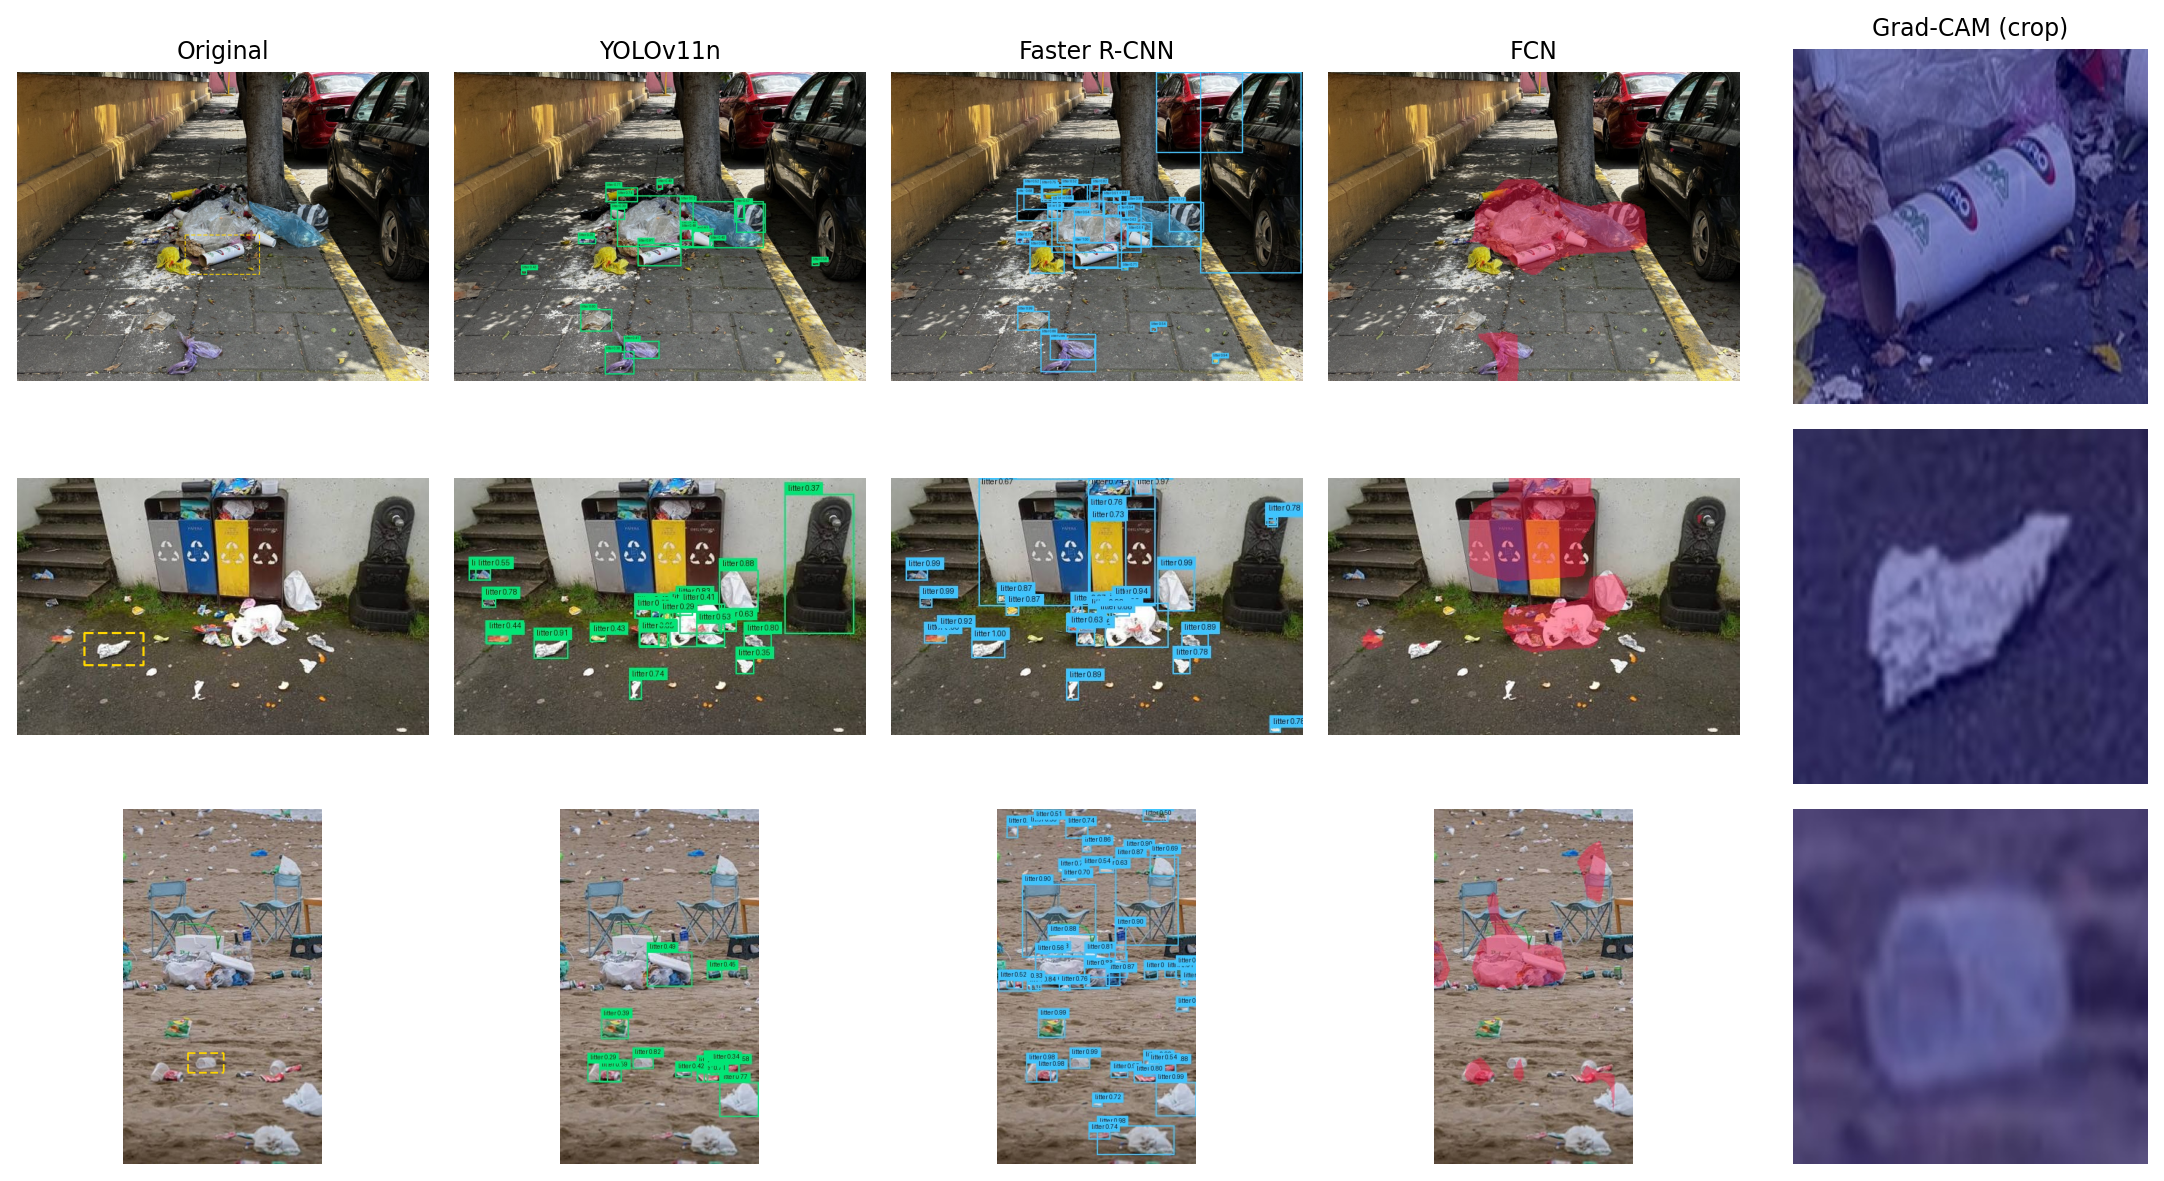
\includegraphics[width=\textwidth]{demo_cualitativa.png}
\caption{Qualitative demo on out-of-distribution web images (three of the ten
in the session): original with the Grad-CAM crop origin marked with a dashed
box, YOLOv11n and Faster R-CNN detections, FCN litter mask and the crop
classifier's Grad-CAM explanation. Images randomly downloaded from the
internet, with no embedded authorship metadata, used for illustration only;
they will be replaced by our own captures (Lima) in a future revision.}
\label{fig:demo}
\end{figure*}

% =============================================================
\section{Discussion and Limitations}
Three findings organize the evidence. \textbf{Litter detectors do not travel.}
The 82\% cross-domain drop, with dashcam isolated and handheld$\leftrightarrow$
drone partially compatible, is explained primarily by object scale: domains
whose object sizes fall within the pretraining anchor range exchange some
knowledge; the 22-px dashcam regime exchanges none. For municipal deployments
mixing sensors, per-domain fine-tuning or at minimum resolution
adaptation remains mandatory; a single universal litter model is not yet
realistic. \textbf{Split hygiene changes conclusions.} The official RoLID
protocol rewards scene memorization (+21\% AP$_{50}$); results published on it
are optimistic by roughly that margin, and the fix (group-aware, by-video
splitting) costs nothing. We argue dataset releases with video or burst
structure should ship group identifiers. \textbf{The cheap levers work.}
1024-px input buys back +8.3 AP$_{50}$ on dashcam; a 2.6\,M-parameter detector
performs within a few points of a 41.3\,M one on single-class litter detection;
and TIDE locates the multiclass bottleneck in material classification rather
than localization suggesting a decoupled design (class-agnostic detector plus
crop classifier, where our VGG substrate reaches 97.8\% accuracy) over ever
finer detection heads.
Limitations we can already state: absolute mAP in this problem is structurally
low~\cite{trashdet}; our compute budget precluded transformer detectors
(CO-DETR-class) which lead RoLID's in-domain benchmark; StreetView-Waste could
not be included (endpoints unavailable); our own OOD capture (Lima) remains
future work, as does temporal aggregation over dashcam video natural given the
video-level structure our audit exposed.

% =============================================================
\section{Conclusion}
We audited three public litter datasets, released corrected group-aware splits,
and measured under a single evaluation contract how far litter detectors
travel across handheld, dashcam and drone imagery. The answers are concrete: an
82\% mAP$_{50}$ drop out of domain with dashcam fully isolated; a +21\%
AP$_{50}$ inflation hiding in RoLID-11K's official splits; up to +8.3
AP$_{50}$ recoverable by input resolution alone; and a 16$\times$ smaller
modern detector within a few points of Faster R-CNN on single-class litter.
Error decomposition shows the remaining battles are background discrimination
and material classification, not localization. The full pipeline from
checksummed ingestion to generated tables plus weights and a live demo are
public; transformer detectors, temporal aggregation over dashcam video and our
planned Lima out-of-distribution capture are the natural next steps.

\section*{Reproducibility}
Code, notebooks (ingest to evaluation), audited splits and trained weights
are released; three reproduction routes are documented (demo
with pretrained weights, metric regeneration from released artifacts in
$\sim$10 minutes, and full retraining from public data). Datasets are downloaded
from their official sources with checksum verification.

\bibliographystyle{IEEEtran}
\bibliography{refs}

\end{document}
